\begin{figure}[ht]
    \centering
    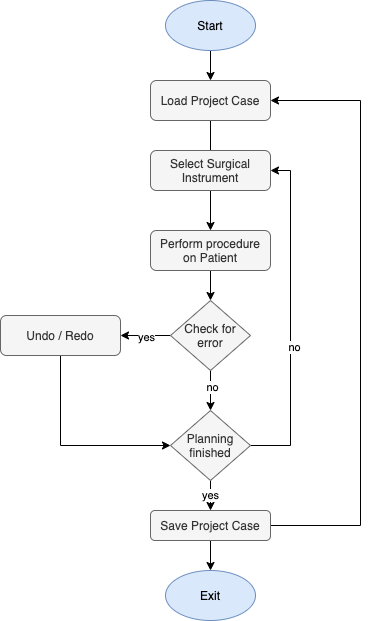
\includegraphics[width=200px]{images/implementation/interaction_flow.png}
    \caption{\label{fig::InteractionFlow}Simplified flow of interaction during the planning stage.}
\end{figure}

The basic flow of interaction for planning a procedure via the software is depicted in Figure \ref{fig::InteractionFlow}.

\textbf{Step 1}: The user has to enable the graphical user interface via the click of a button on the controller.
The user interface will be stuck to the left hand of the user, another click of the button will freeze the GUI in place.
The user interacts with the graphical interface by perfoming virtual button presses with his virtual hands.
Via the interface, the user first chooses a project case he wants to work on.
This will load the patient data into the virtual operating room, ready for planning the procedure via the available tools.
From here on, the user can freely choose which procedure to perform and in which order.
\\
\textbf{Step 2}: Tools are selected by simply walking or teleporting to them and making a natural grab motion via the gesture interface of the system.
\\
\textbf{Step 3}: When holding a surgical instrument, the perform action has to be executed to add a procedure step.
By simply touching the respective button, the user gets a visual indication that a procedure is about to be performed.
When performing a procedure step, the user gets auditory feedback that the step has been registered.
At any point of performing the procedure, the user can choose to undo and redo the current step via the VUI.
Only the last performed step will be visible while planning the procedure for visibility reasons.
\\
\textbf{Step 4}: When a procedure has been planned and the project case has been finished, the user has to save the project via the GUI.
This will create a copy of the current patient model including all procedure steps and save it to the users hard drive.
